\subsection{Microcontrolador}
En base a los sensores seleccionados y los requerimientos del proyecto, seconsideraron los siguientes microcontroladores:
\begin{landscape}
\begingroup
\setlength{\tabcolsep}{5pt} % Reduce el espacio entre columnas
\renewcommand{\arraystretch}{1.5} % Aumenta la altura de las filas
\begin{longtable}{|p{2.5cm}|p{2.5cm}|p{2.5cm}|p{2.5cm}|p{2cm}|p{2cm}|p{1.5cm}|m{2cm}|}
\caption{Microcontroladores}
\label{tab:microcontroladores}
\\
\hline
\textbf{Modelo} & \textbf{Procesador / Frecuencia} & \textbf{Memoria} & \textbf{Conectividad} & \textbf{Puertos} & \textbf{Voltaje de Operación} & \textbf{Precio (USD)} & \textbf{Imagen} \\
\hline
\endfirsthead
\hline
\textbf{Modelo} & \textbf{Procesador / Frecuencia} & \textbf{Memoria} & \textbf{Conectividad} & \textbf{Puertos} & \textbf{Voltaje de Operación} & \textbf{Precio (USD)} & \textbf{Imagen} \\
\hline
\endhead
\hline
\endfoot
\endlastfoot

XIAO ESP32C6 \cite{zotero-item-58} & RISC-V 32-bit Single-Core / 160 MHz & ROM 320KB, SRAM 512KB, Flash 4MB & Wi-Fi 6, BLE 5, Zigbee 3.0, Thread & 1xI2C, 1xUART, 1xSPI, 1xI2S, 11xGPIO & 3.3V (5V VCC) & $\sim$7 & 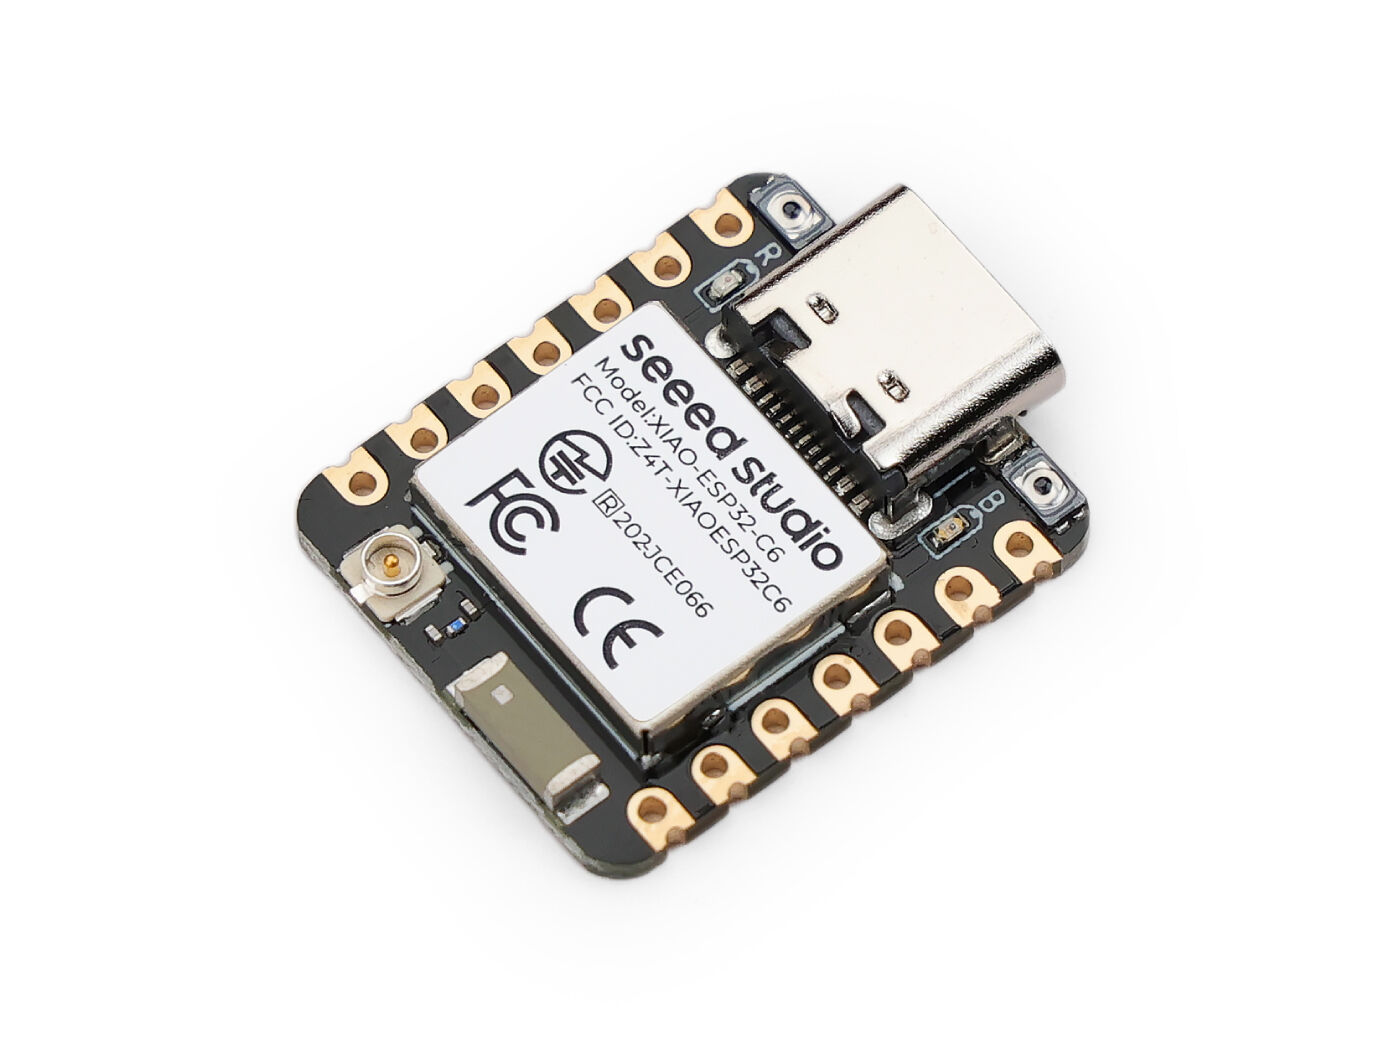
\includegraphics[width=20mm]{./Imagenes/Módulo1/Microcontrolador/1-113991254-seeedxiao-esp32c6-45font_1.jpg}\\
\hline
ESP32-C3 SuperMini \cite{K} & RISC-V 32-bit Single-Core / 160 MHz & ROM 400KB, SRAM 400KB, Flash 4MB & Wi-Fi 4 (802.11n), BLE 5 & 2xUART, 2xI2C, 1xSPI, 13xGPIO & 3.3V (5V VCC) & $\sim$4 &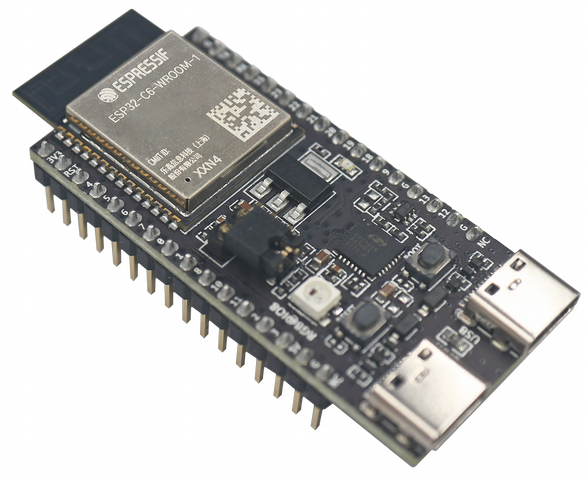
\includegraphics[width=20mm]{./Imagenes/Módulo1/Microcontrolador/esp32-c6.png} \\
\hline
ESP32-H2M-1 (Módulo) \cite{zotero-item-61} & RISC-V 32-bit Single-Core / 96 MHz & ROM 320KB, SRAM 256KB, Flash 4MB & BLE 5, Zigbee 3.0, Thread & 1xSPI, 2xUART, 1xI2C, 1xI2S, 18xGPIO & 3.3V & $\sim$3 & 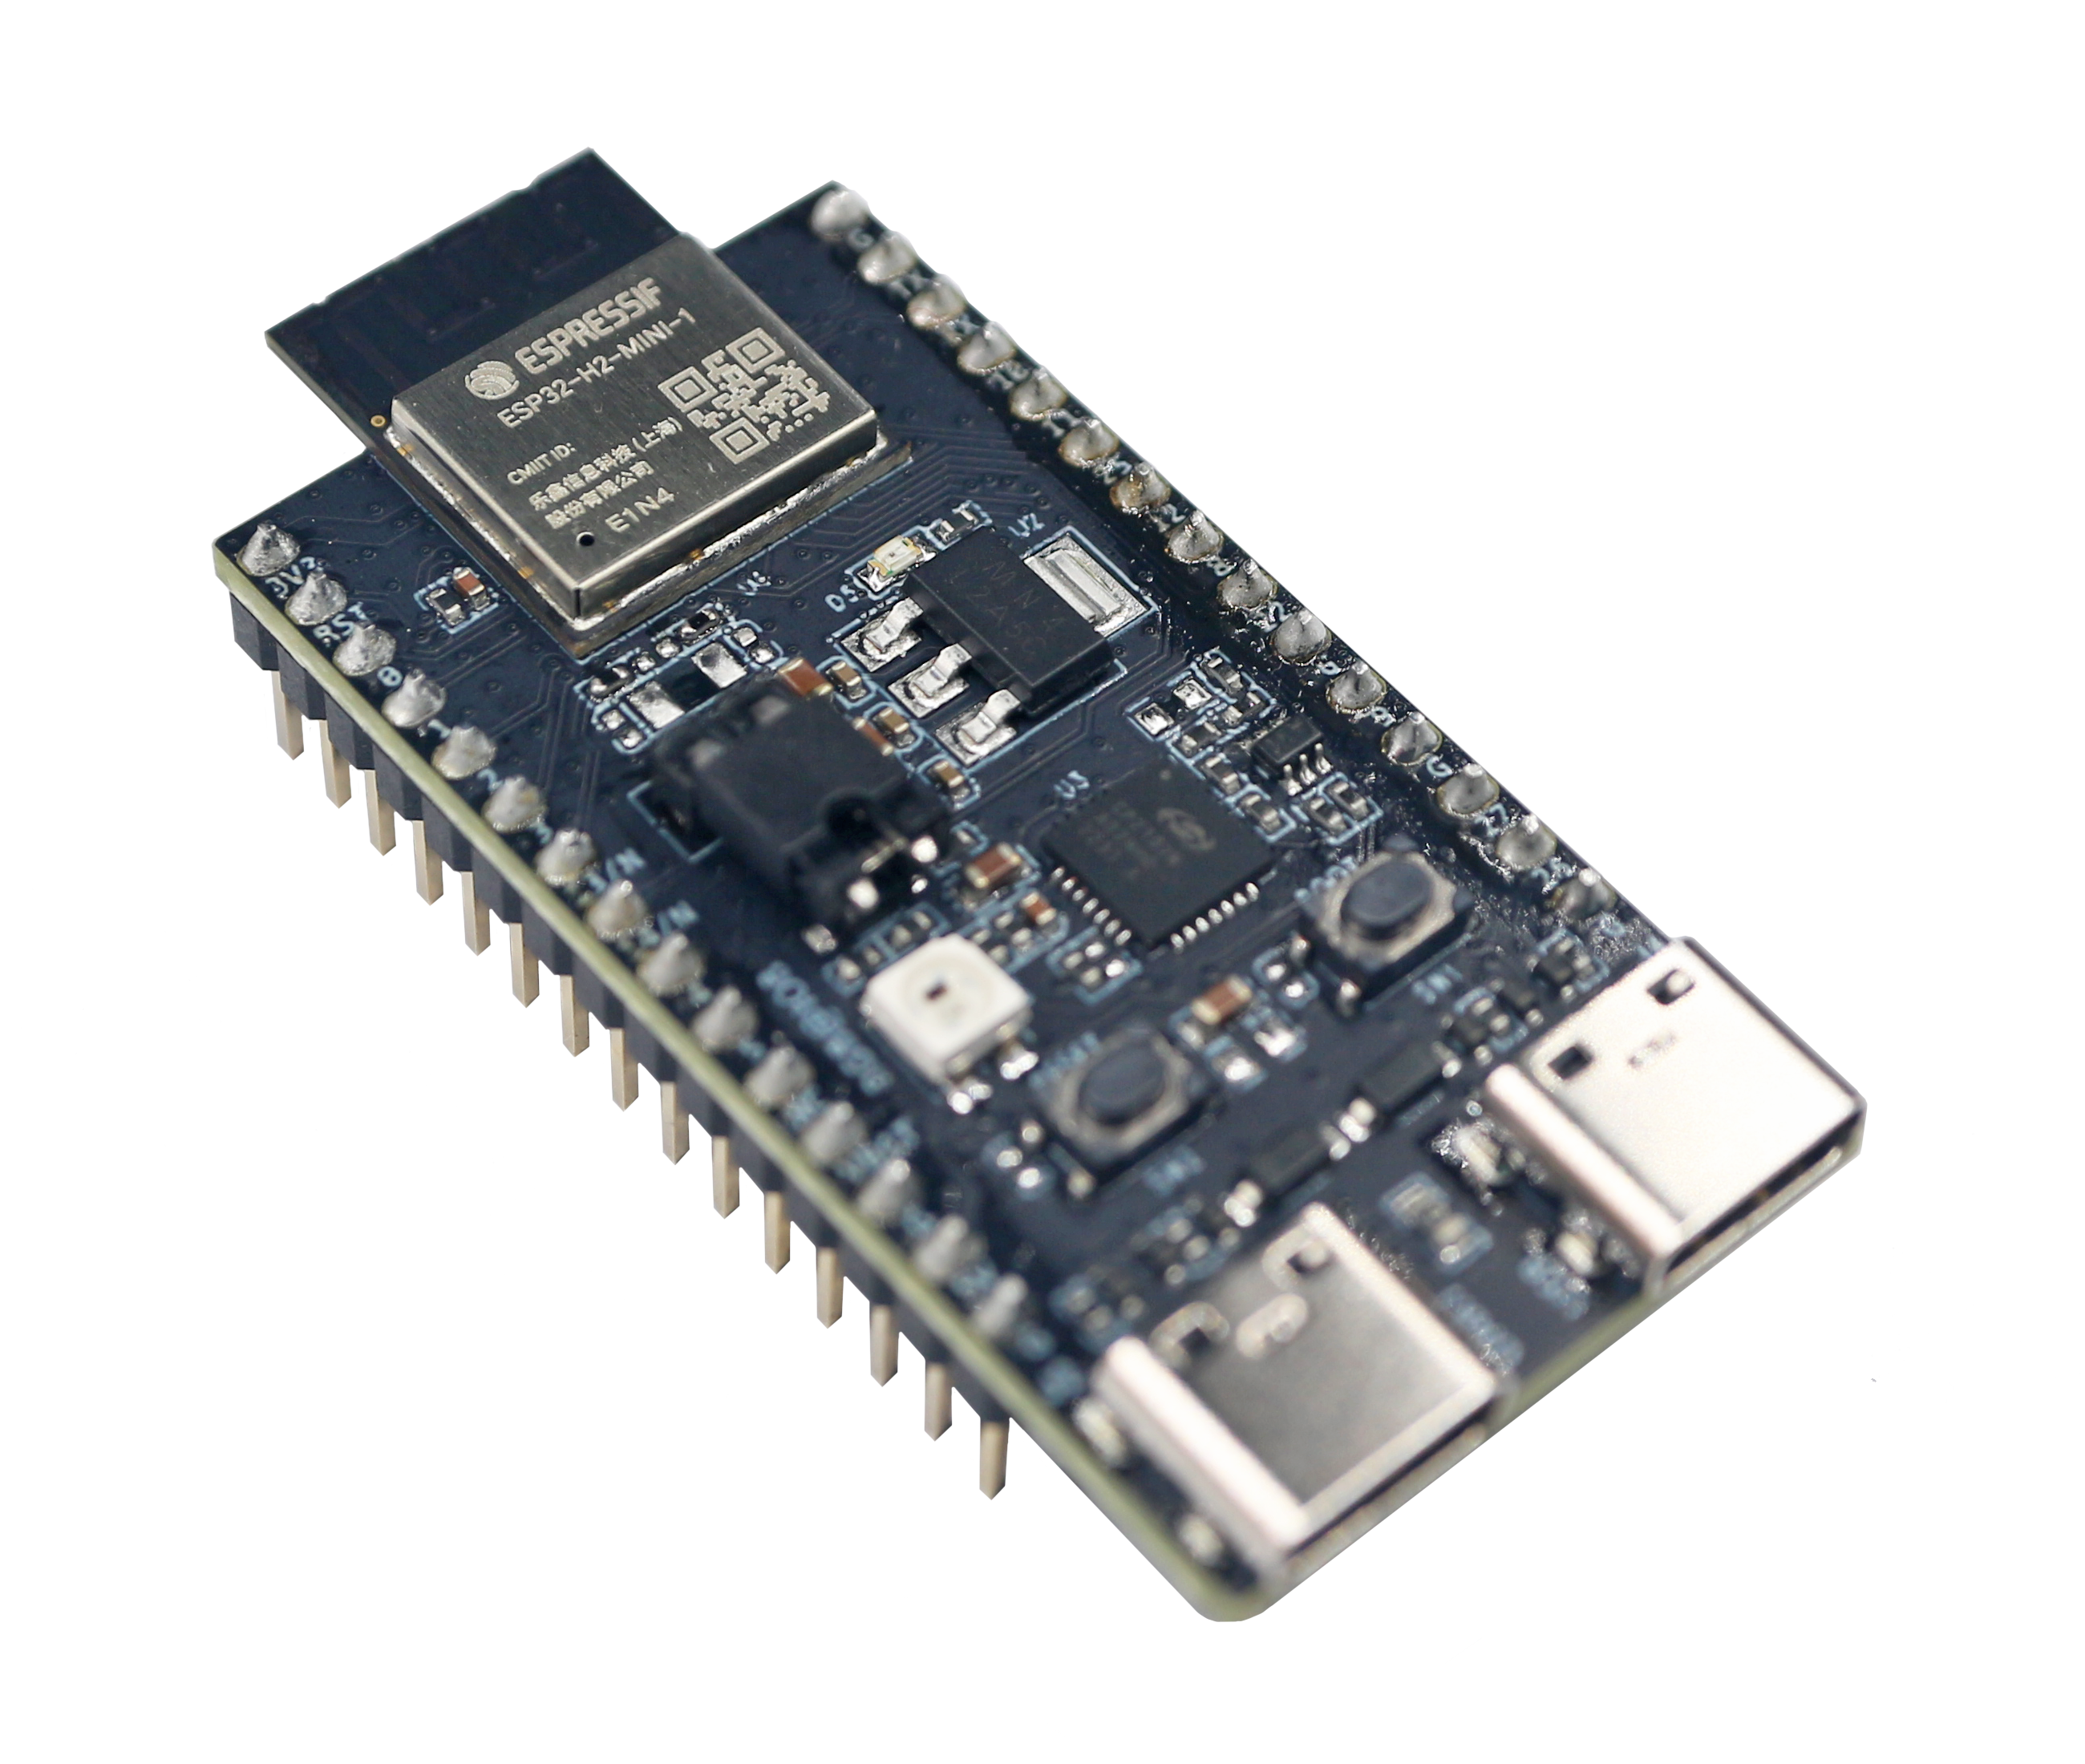
\includegraphics[width=20mm]{./Imagenes/Módulo1/Microcontrolador/esp32-h2-devkitm-1-45-20230303.png}\\
\hline
ESP32-C6-DEVKITC-1-N8 \cite{zotero-item-62}& RISC-V 32-bit Single-Core / 160 MHz & ROM 320KB, SRAM 512KB, Flash 8MB & Wi-Fi 6, BLE 5, Zigbee 3.0, Thread & 4xSPI, 3xUART, 2xI2C, 2xI2S, 23xGPIO & 3.3V (5V Micro-USB) & $\sim$8 & 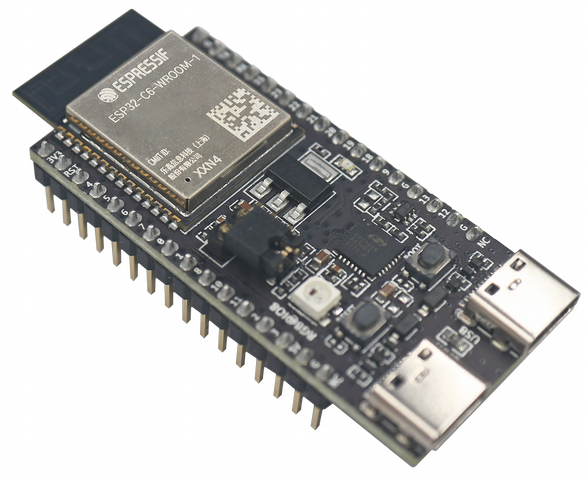
\includegraphics[width=20mm]{./Imagenes/Módulo1/Microcontrolador/esp32-c6.png}\\
\hline
ESP32-DevKitC-32E \cite{Embajadores} & Xtensa LX6 Dual-Core / 240 MHz & ROM 448KB, SRAM 520KB, Flash 4MB & Wi-Fi 4 (802.11n), BT 4.2 & 3xSPI, 3xUART, 2xI2C, 2xI2S, 34xGPIO & 3.3V (5V Micro-USB) & $\sim$6 & 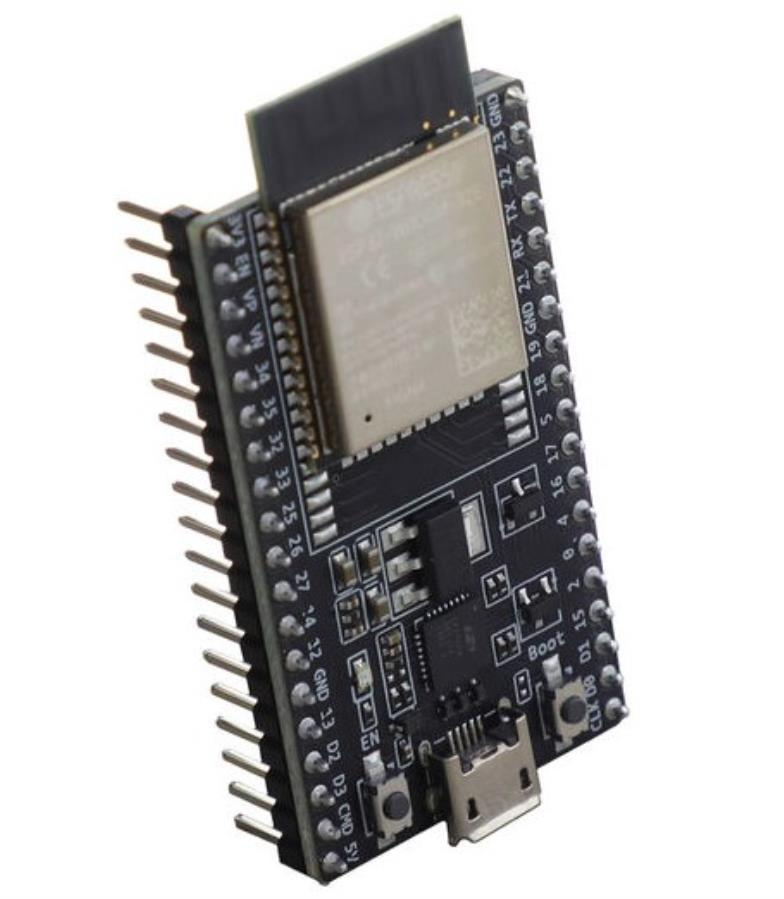
\includegraphics[width=20mm]{./Imagenes/Módulo1/Microcontrolador/esp32.jpg}\\
\hline
ESP32-C2 (Módulo) \cite{zotero-item-52}& RISC-V 32-bit Single-Core / 120 MHz & ROM 320KB, SRAM 272KB, Flash 4MB & Wi-Fi 4 (802.11n), BLE 5 & 2xSPI, 2xUART, 1xI2C, 1xI2S, 14xGPIO & 3.3V & $\sim$2 & 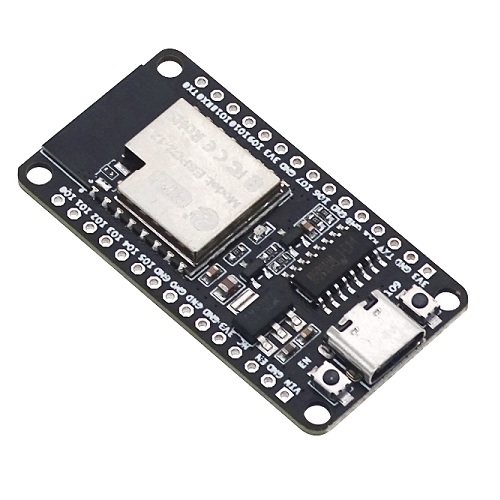
\includegraphics[width=20mm]{./Imagenes/Módulo1/Microcontrolador/c2.jpg}\\
\hline
Raspberry Pi Pico 2 W \cite{zotero-item-68}& ARM Cortex M0+ Dual-Core / 133 MHz & SRAM 264KB, Flash 4MB & Wi-Fi 4 (802.11n), BT 5.2 & 2xSPI, 2xI2C, 2xUART, 16xPWM, 26xGPIO & 3.3V (5V Micro-USB) & $\sim$6 & 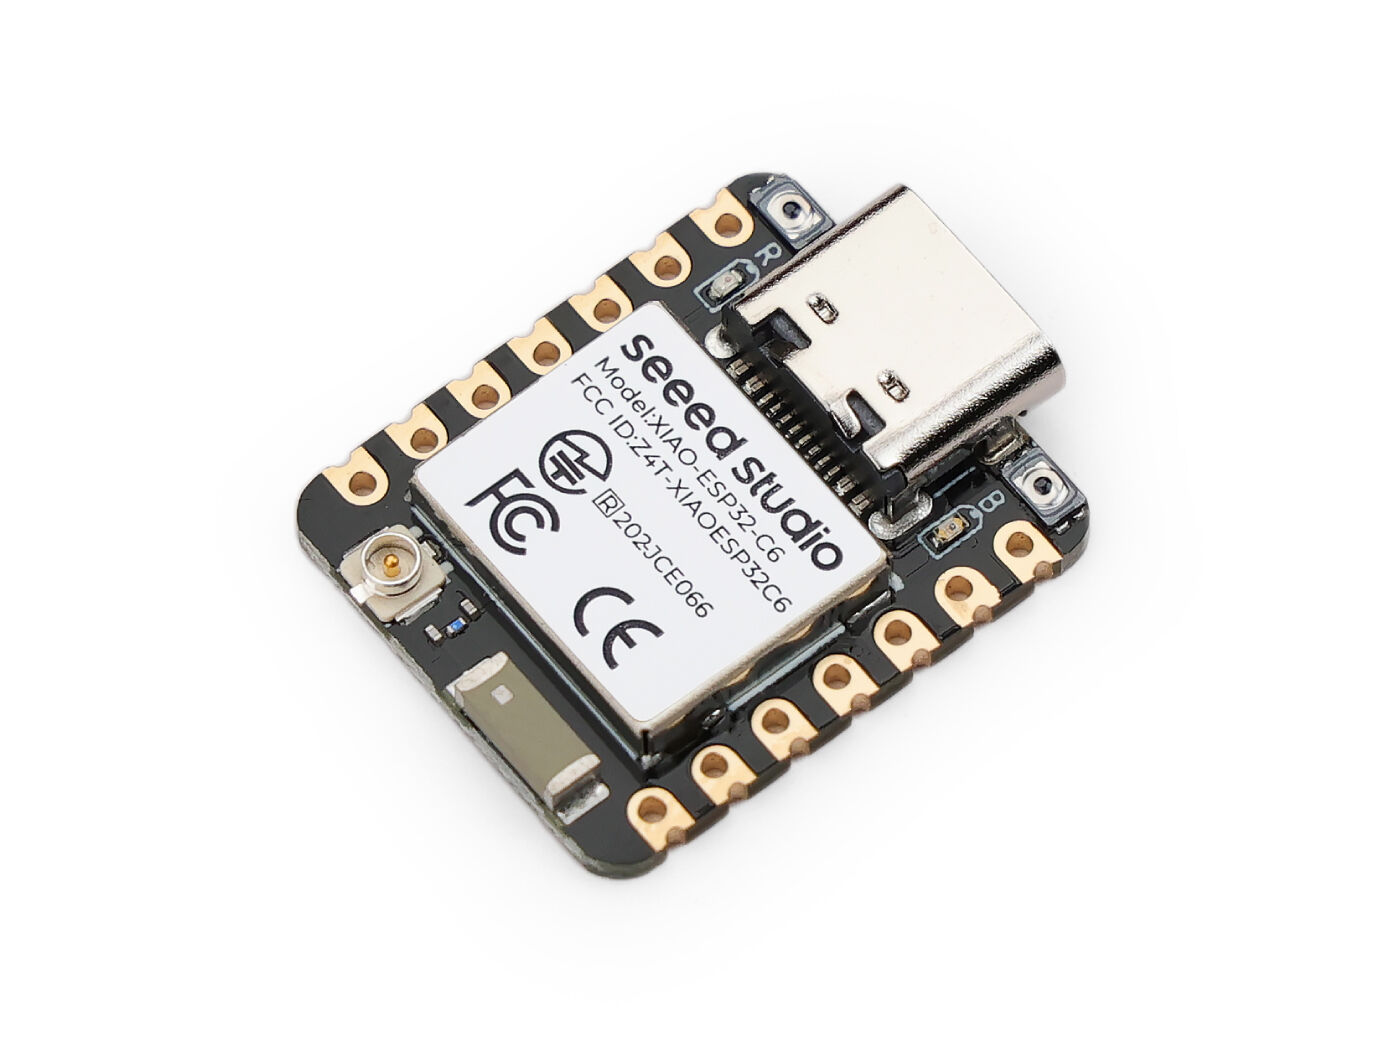
\includegraphics[width=20mm]{./Imagenes/Módulo1/Microcontrolador/1-113991254-seeedxiao-esp32c6-45font_1.jpg}\\
\hline
Raspberry Pi Pico 2 WH \cite{zotero-item-68} & ARM Cortex M0+ Dual-Core / 133 MHz & SRAM 264KB, Flash 4MB & Wi-Fi 4 (802.11n), BT 5.2 & 2xSPI, 2xI2C, 2xUART, 16xPWM, 26xGPIO & 3.3V (5V Micro-USB) & $\sim$8 & 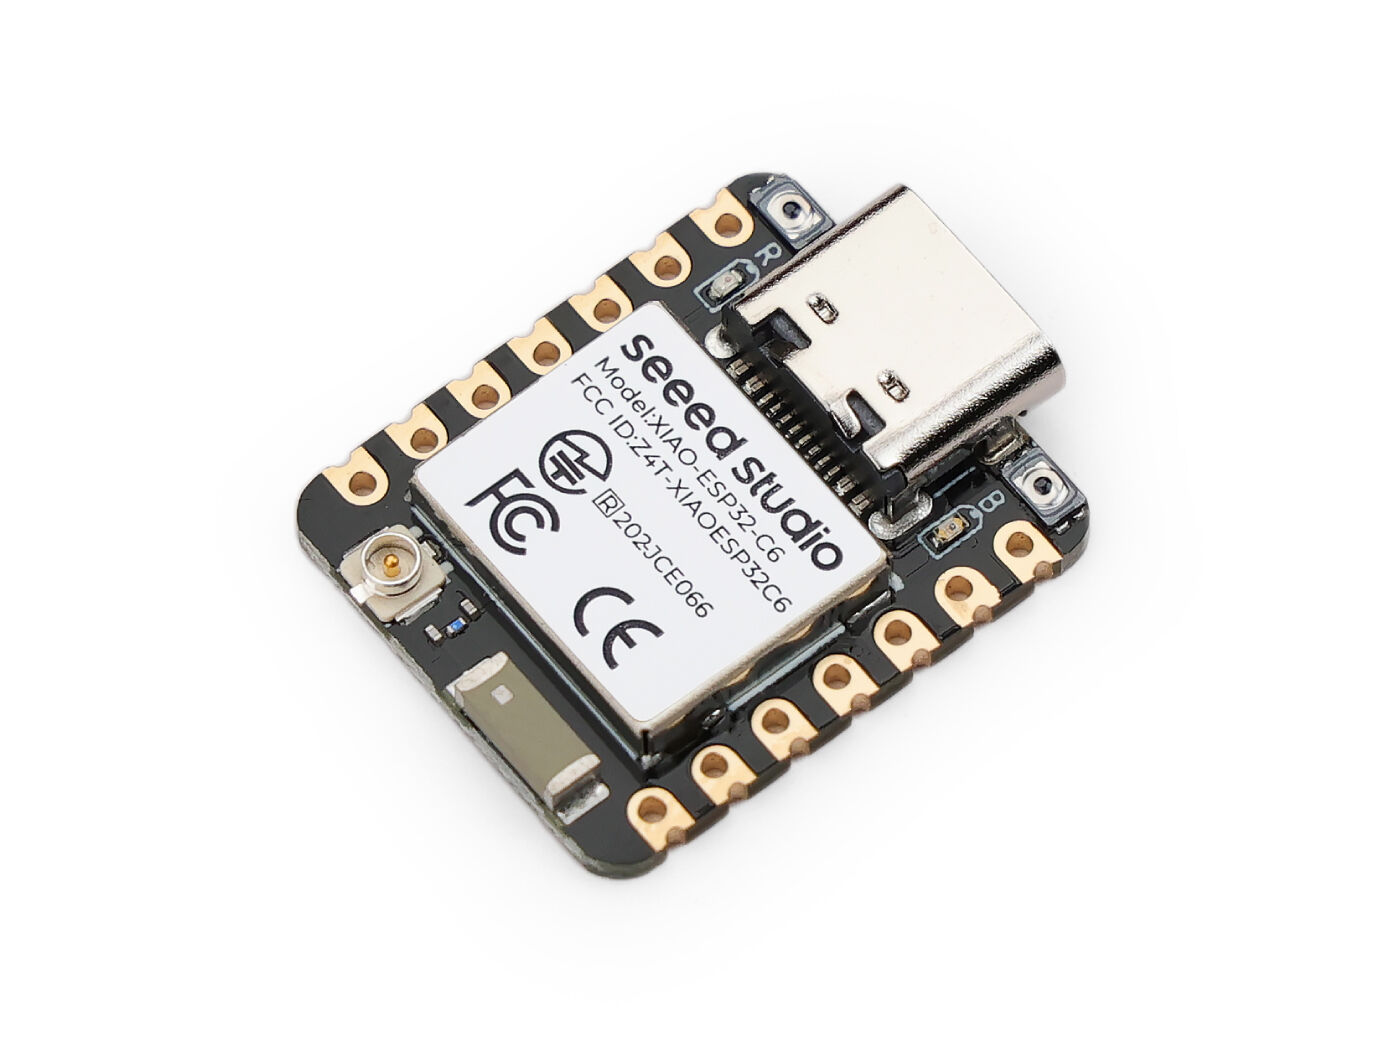
\includegraphics[width=20mm]{./Imagenes/Módulo1/Microcontrolador/1-113991254-seeedxiao-esp32c6-45font_1.jpg}\\
\hline
\end{longtable}
\endgroup
\end{landscape}



\subsection{Fuente de alimentación}

\section{Análisis del Módulo 2}
Para llevar acabo el analisis de datos en base a los requerimientos funcionales se 
consideran los siguientes lenguajes:
\begin{table}[h]
    \centering
    \caption{Comparativa de Lenguajes para Lógica Difusa y JSON}
    \label{tab:lenguajes_fuzzy}
    \begin{tabular}{|l|c|c|c|l|}
        \hline
        \textbf{Lenguaje} & \textbf{Adecuación para Lógica Difusa} & \textbf{Librería Principal} & \textbf{Manejo de JSON} & \textbf{Uso Típico en el Proyecto} \\
        \hline
        \textbf{Python} & Excelente & \texttt{scikit-fuzzy} & Excelente (Nativo) & Backend de Análisis, API, y lógica difusa \\
        \hline
        \textbf{R} & Adecuada/Buena & \texttt{sets}, \texttt{FuzzyR} & Buena (Con \texttt{jsonlite}) & Análisis Estadístico Avanzado \\
        \hline
        \textbf{C\#} & Adecuada & \texttt{FuzzyLogic}, \texttt{FuzzySharp} & Muy Buena (Nativo con \texttt{System.Text.Json}) & Aplicaciones de Escritorio/Servidor (.NET) \\
        \hline
    \end{tabular}
\end{table}
\section{Análisis del Módulo 3}
Para llevar acabo el analisis de datos en base a los requerimientos funcionales se 
consideran los siguientes lenguajes:
\begin{table}[h]
    \centering
    \caption{Resumen de Bases de Datos para Proyectos IoT}
    \label{tab:bd_resumen}
    \begin{tabular}{|l|l|l|l|}
        \hline
        \textbf{Característica} & \textbf{InfluxDB (Series de Tiempo)} & \textbf{PostgreSQL (Relacional)} & \textbf{MongoDB (Documentos)} \\
        \hline
        \textbf{Uso Principal en IoT} & Datos de Sensores (pH, Temp, etc.) & Gestión de Usuarios y Metadatos & Datos Semiestructurados \\
        \hline
        \textbf{Optimización TS*} & \textbf{Excelente} (Diseño Nativo) & Baja (Requiere Extensiones) & Baja (No Optimizado) \\
        \hline
        \textbf{Manejo de JSON} & Muy Buena (API y Formato) & \textbf{Excelente} (\texttt{jsonb} Nativo) & \textbf{Excelente} (Formato Nativo) \\
        \hline
        \textbf{Flexibilidad Esquema} & Baja (Esquema Fijo) & Baja (Esquema Estricto) & \textbf{Excelente} (Esquema Dinámico) \\
        \hline
        \textbf{Escalabilidad} & Alta & Media-Alta & \textbf{Alta} \\
        \hline
        \multicolumn{4}{l}{\small *TS: Series de Tiempo} \\
    \end{tabular}
\end{table}
\section{Análisis del Módulo 4}
En esta sección se presenta un análisis comparativo de las opciones de frontend para el monitoreo del sistema IoT, considerando las necesidades específicas del proyecto, como la visualización de datos en tiempo real, la personalización de la interfaz y la integración con la base de datos InfluxDB.
Se evaluaron dos opciones principales: Grafana y un framework de desarrollo web como React o Vue
\begin{table}[h]
    \centering
    \caption{Resumen de Opciones de Frontend para Monitoreo IoT}
    \label{tab:frontend_resumen}
    \begin{tabular}{|l|l|l|l|}
        \hline
        \textbf{Característica} & \textbf{Grafana}  & \textbf{React (o Vue.js)}  & \textbf{Apto para tu Proyecto} \\
        \hline
        \textbf{Tipo de Solución} & Herramienta de Visualización & Framework de Desarrollo & \\
        \hline
        \textbf{Personalización de UI} & Limitada (Paneles y Plugins) & \textbf{Total} & \multicolumn{1}{l|}{} \\
        \hline
        \textbf{Integración con InfluxDB} & \textbf{Nativa y Directa} & Vía \textbf{Backend API} & \multicolumn{1}{l|}{} \\
        \hline
        \textbf{Gestión de Usuarios Específica} & Requiere Plugins/Configuración Compleja & \textbf{Ideal} (Manejada por Backend) & \multicolumn{1}{l|}{} \\
        \hline
        \textbf{Velocidad de Desarrollo} & \textbf{Rápida} (Dashboard Básico) & Lenta (Aplicación Completa) & \multicolumn{1}{l|}{} \\
        \hline
        \textbf{Recomendación} & Pruebas y Visualización Básica & \textbf{Desarrollo de Aplicación Completa} & \textbf{React (o Vue.js)} \\
        \hline
    \end{tabular}
\end{table}
\section{Framework}
En esta sección se presenta un análisis comparativo de los principales frameworks de backend en Python, evaluando su idoneidad para el desarrollo de una API RESTful que maneje la lógica del sistema IoT, la comunicación con la base de datos InfluxDB y la gestión de usuarios.
\begin{table}[h]
    \centering
    \caption{Resumen de Frameworks de Backend de Python para IoT}
    \label{tab:backend_resumen}
    \begin{tabular}{|l|l|l|l|}
        \hline
        \textbf{Característica} & \textbf{FastAPI}  & \textbf{Flask}  & \textbf{Django} \\
        \hline
        \textbf{Tipo de Framework} & Asíncrono (API-first) & Microframework & Full-Stack \\
        \hline
        \textbf{Rendimiento} & \textbf{Excelente} (El más rápido) & Bueno & Aceptable \\
        \hline
        \textbf{Lógica Asíncrona} & \textbf{Nativa} (Ideal para MQTT) & Requiere Ext. & Requiere Config. \\
        \hline
        \textbf{Gestión de Usuarios} & Requiere Desarrollo Manual & Requiere Ext. & \textbf{Integrada} \\
        \hline
        \textbf{Documentación API} & \textbf{Automática (Swagger/OpenAPI)} & Requiere Ext. & Requiere Ext. \\
        \hline
        \textbf{Curva de Aprendizaje} & Media & \textbf{Baja} & Alta \\
        \hline
        \textbf{Recomendación para IoT} & \textbf{Mejor Opción} (Rendimiento y API) & Buena Opción (Simplicidad) & No Recomendado (Sobrecarga) \\
        \hline
    \end{tabular}
\end{table}
\section{Servidor}




